\documentclass{myslide}
\author{M. Pulido}
\date{\today}
\title{Implementacion NNs para regresion}
\hypersetup{
 pdfauthor={M. Pulido},
 pdftitle={Implementacion NNs para regresion},
 pdfkeywords={},
 pdfsubject={},
 pdfcreator={Emacs 27.2 (Org mode 9.5.2)}, 
 pdflang={English}}
\begin{document}
\begin{frame}
\maketitle
%\tableofcontents
\end{frame}

\begin{frame}{Entrenamiento red  neuronal para regresion. Caso teorico}

Dado \(z\) quiero estimar \(x\), en particular su media \(\mu_x\)  y su desviacion standard \(\sigma_x\).

Es decir la red neuronal debe predecir una Gaussiana parametricamente.

\rp{Arquitectura de la red:}  FCNN (Hidden 64x32), activation function GELU (smooth ReLU). 

\rp{Funcion de perdida:} Necesitamos sensibilidad a \(\sigma_x\)

\begin{itemize}
\item Negativo de la log verosimilitud  $ - log L = - log \prod_j^N p(x_j|z_j) =   \frac{N}{2} \log \sigma(z)^2  \frac{1}{2\sigma(z)²} \sum_{j=1}^N \left(x - \mu_x\right)^2$  
\item Extended MSE:  $ (1-\lambda) (x-\mu_x(z))^2 + \lambda \left[\sigma_x(z)^2 -  (x-\mu_x(z))^2 \right]^2$ donde $(x-\mu_x)^2$ son los residuales o error de prediccion (de la media).
\end{itemize}

\end{frame}


\begin{frame}{Entrenamiento Log-likelihood}

\label{sec:org7ca273e}

\begin{center}
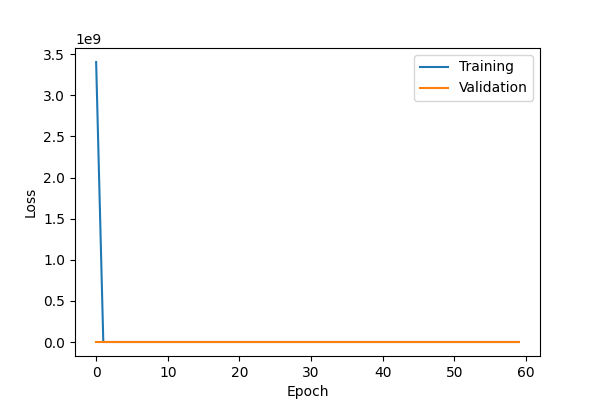
\includegraphics[width=.50\linewidth]{./fig/loss_sin_llik.png}
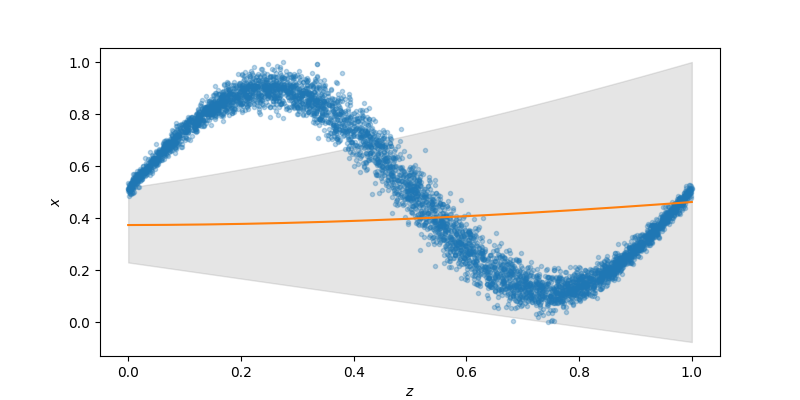
\includegraphics[width=.60\linewidth]{./fig/prediction_sin_llik.png}
\end{center}

\end{frame}

\begin{frame}{Mixed MSE - Log-likelihood}

  Se empieza entrenando con MSE y gradualmente se empieza a dar peso a la Log-likelihood
  
\begin{center}
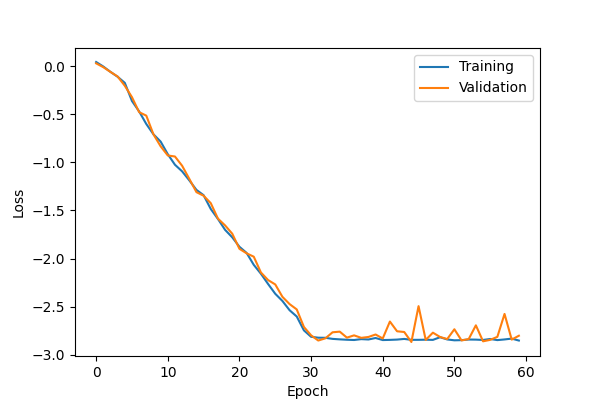
\includegraphics[width=.50\linewidth]{./fig/loss_sin_mixtaLlik.png}
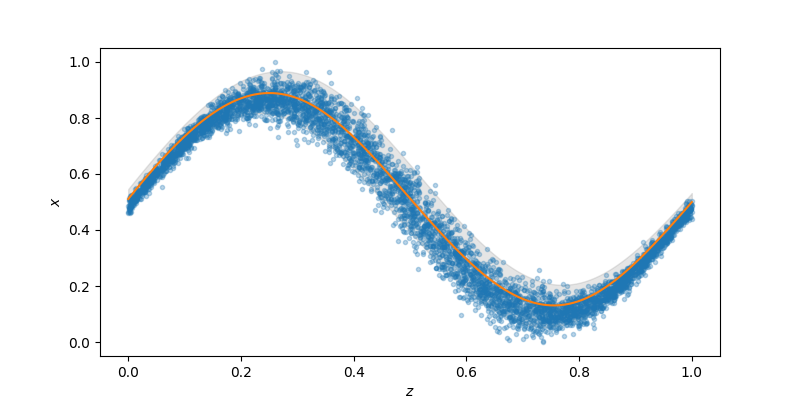
\includegraphics[width=.60\linewidth]{./fig/prediction_sin_mixtaLlik.png}
\end{center}

\end{frame}
\begin{frame}{Mixed MSE - eMSE}


  Se empieza entrenando con MSE y gradualmente se empieza a dar peso a la prediccion del error
 
\begin{center}
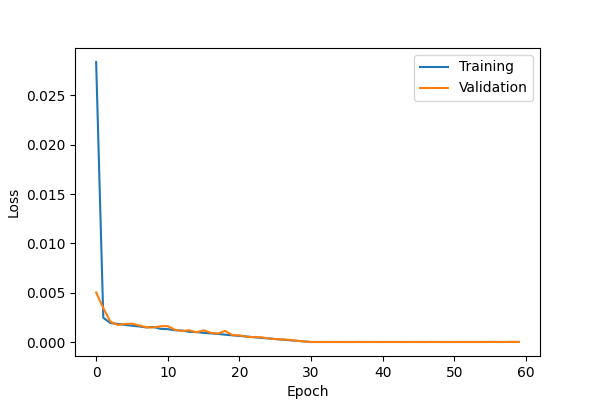
\includegraphics[width=.50\linewidth]{./fig/loss_sin_mixed_emse.png}
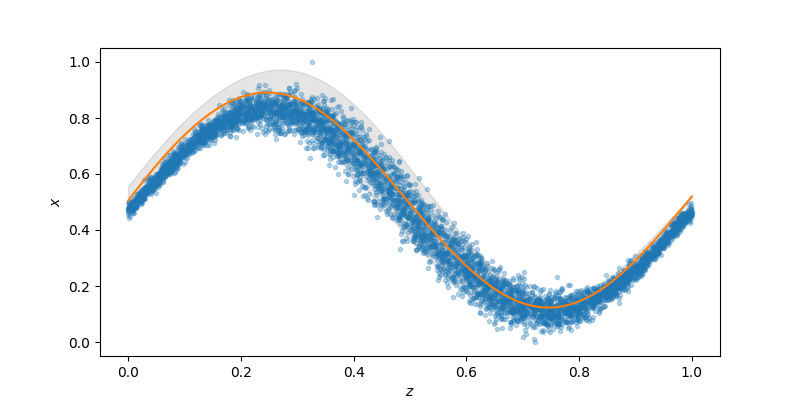
\includegraphics[width=.60\linewidth]{./fig/prediction_sin_mixed_emse.png}
\end{center}

\end{frame}
\begin{frame}{Red neuronal para activos sinteticos}

Usando Mixed MSE  - Log-lik como funcion de perdida

%\vskip -0.2cm
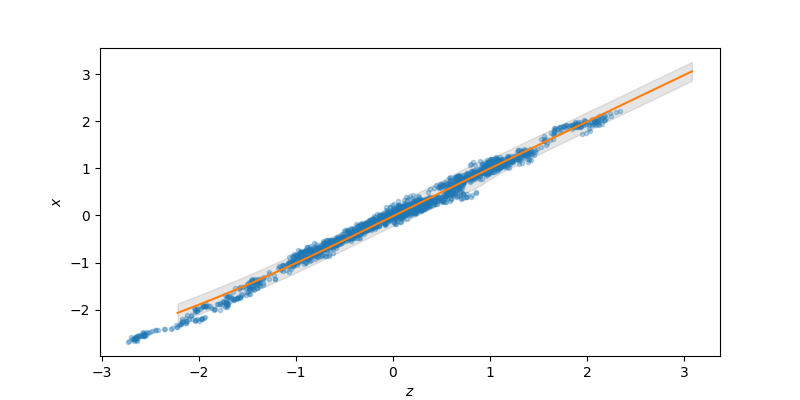
\includegraphics[width=.65\linewidth]{./fig/prediction_syn_assets_mixed_nll.png}
%\vskip -0.3cm
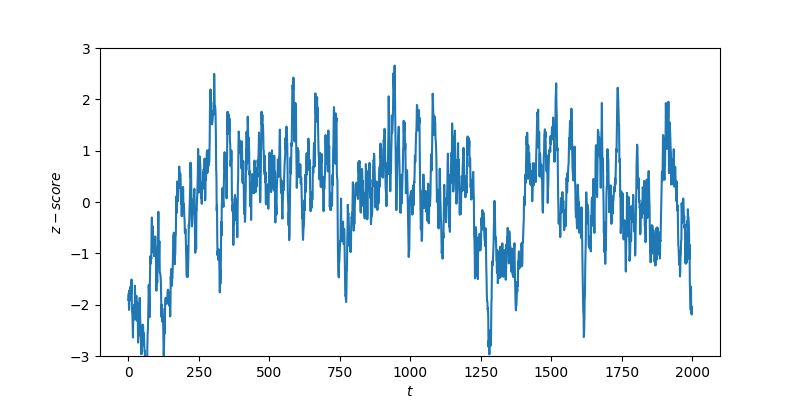
\includegraphics[width=.65\linewidth]{./fig/zcore_syn_assets_mixed_nll.png}

\end{frame}

\begin{frame}{Usando Mixed MSE - Extended-MSE}
%\vskip -0.2cm
  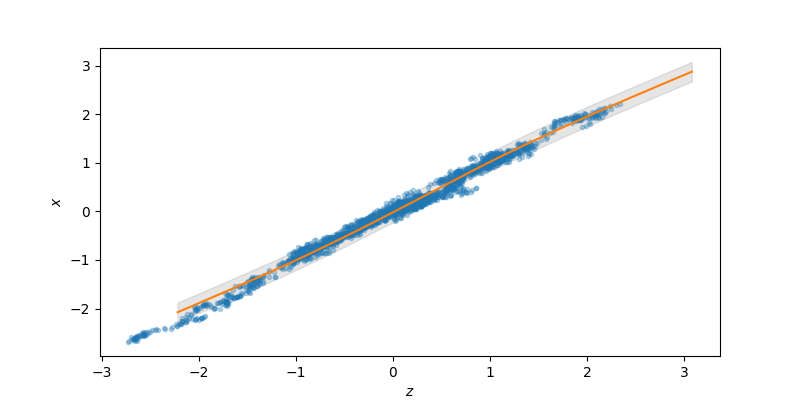
\includegraphics[width=.70\linewidth]{./fig/prediction_syn_assets_mixed_emse.png}
%\vskip -0.3cm
  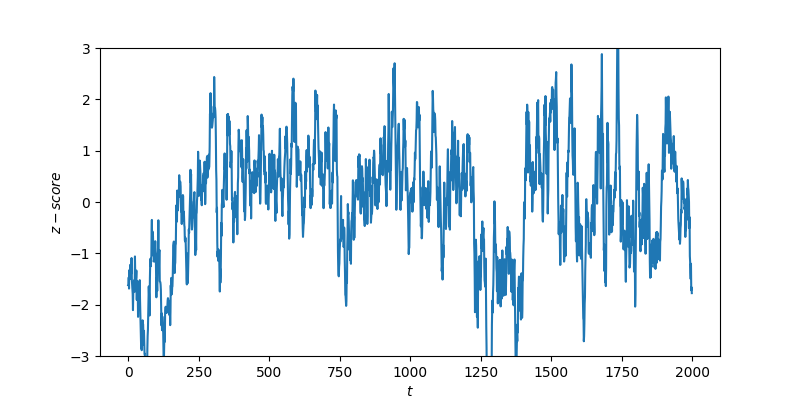
\includegraphics[width=.70\linewidth]{./fig/zcore_syn_assets_mixed_emse.png}

\end{frame}

\begin{frame}{Transporte optimo como distancia entre distribuciones}

Tenemos una muestra sintetica (generada por una distribucion propuesta) y tenemos la muestra de los datos. 

Concepto. Queremos medir cuan distintas son las muestras.

Para estos se transportan las muestras sinteticas hasta las muestras de los datos  (seleccionando pares cercanos) y se mide la distancia de esos transportes.


\rp{Nos permite saber cuan bueno es nuestro modelo, o de dos modelos cual es superior en terminos probabilisticos}

\end{frame}
\begin{frame}{Comparacion de copulas usando transporte optimo}
\begin{center}
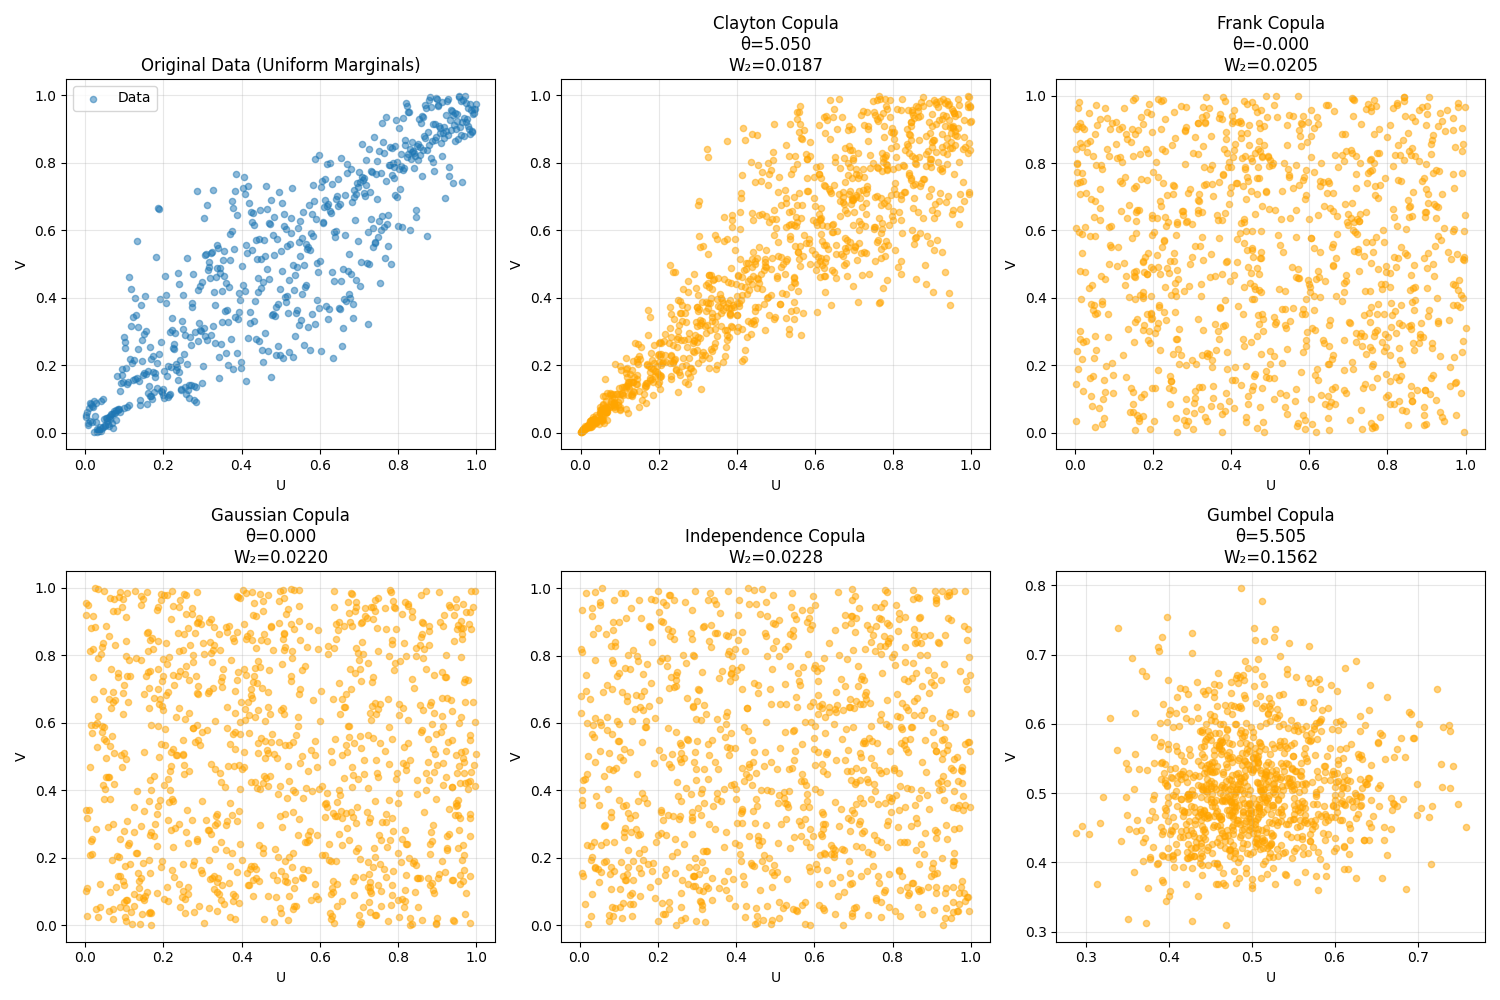
\includegraphics[width=.9\linewidth]{./fig/copulas-ot.png}
\end{center}
Datos: Activos sinteticos.
\end{frame}

\end{document}
